\documentclass[10pt,letterpaper]{article}

%% our packages %%
\usepackage{multirow}
\usepackage{multicol}
\usepackage{longtable}
\usepackage{amssymb}
\usepackage{paralist}
\usepackage{times}
\usepackage{pbox}
\topmargin 0.0cm
\oddsidemargin 0.2cm
\textwidth 16cm 
\textheight 21cm
\usepackage{setspace}
%\usepackage{subfigure}
\usepackage{graphicx}
\usepackage{algorithm}
\usepackage{algorithmic}
%\usepackage{natbib}
\usepackage{units}
\usepackage{microtype}
\usepackage{appendix}
\usepackage{hyperref}
\usepackage{color}
%\usepackage{spacing}
\usepackage{units}
\usepackage{microtype}
\usepackage{relsize}
\usepackage{verbatim}
\usepackage{soul}
\definecolor{MyBlue}{rgb}{0.2,0.2,0.8}
\newcommand{\inblue}[1]{{\color{MyBlue}\sf\textbf{\textsc{#1}}}}
\newcommand{\supplementary}[0]{\inblue{[Supplementary Material]}}

\newcommand{\highlight}[1]{\colorbox{yellow}{#1}}
\renewcommand{\algorithmicrequire}{\textbf{Input:}}
\renewcommand{\algorithmicensure}{\textbf{Output:}}
\newcommand{\lw}{\Lambda_{W}}
\newcommand{\lv}{\Lambda_{V}}
\newcommand{\uw}{U_{W}} 
\newcommand{\uv}{U_{V}}
%\newcommand{\tbf}[x]{\textbf{x}}
\newcommand{\ess}{\mathcal{S}}
\renewcommand{\H}{\mathcal{H}}
\renewcommand{\L}{\mathcal{L}}
\newcommand{\I}{\mathcal{I}} 
\renewcommand{\L}{\mathcal{L}}
\newcommand{\G}{\mathcal{G}}
\newtheorem{theorem}{Theorem}
\newtheorem{lemma}{Lemma}
\newcommand{\theHalgorithm}{\arabic{algorithm}}
\usepackage{graphicx}
\footskip 1.0cm
\newenvironment{sciabstract}{%
\begin{quote} \bf}
{\end{quote}}
\renewcommand\refname{References and Notes}
\newcounter{lastnote}
\newenvironment{scilastnote}{%
\setcounter{lastnote}{\value{enumiv}}%
\addtocounter{lastnote}{+1}%
\begin{list}%
{\arabic{lastnote}.}
{\setlength{\leftmargin}{.22in}}
{\setlength{\labelsep}{.5em}}}
{\end{list}}

\usepackage{booktabs}

%%%%%%%%%%%%%%%%%%%%%%



\usepackage[top=0.85in,left=2.75in,footskip=0.75in]{geometry}

% Use adjustwidth environment to exceed column width (see example table in text)
\usepackage{changepage}

% Use Unicode characters when possible
\usepackage[utf8]{inputenc}

% textcomp package and marvosym package for additional characters
\usepackage{textcomp,marvosym}

% fixltx2e package for \textsubscript
\usepackage{fixltx2e}

% amsmath and amssymb packages, useful for mathematical formulas and symbols
\usepackage{amsmath,amssymb}

% cite package, to clean up citations in the main text. Do not remove.
\usepackage{cite}

% Use nameref to cite supporting information files (see Supporting Information section for more info)
\usepackage{nameref,hyperref}

% line numbers
\usepackage[right]{lineno}

% ligatures disabled
\usepackage{microtype}
\DisableLigatures[f]{encoding = *, family = * }

% rotating package for sideways tables
\usepackage{rotating}

% Remove comment for double spacing
%\usepackage{setspace} 
\doublespacing

% allow full width tables
\usepackage{tabularx}

% Text layout
\raggedright
\setlength{\parindent}{0.5cm}
\textwidth 5.25in 
\textheight 8.75in

% Bold the 'Figure #' in the caption and separate it from the title/caption with a period
% Captions will be left justified
\usepackage[aboveskip=1pt,labelfont=bf,labelsep=period,justification=raggedright,singlelinecheck=off]{caption}
\usepackage{subcaption}
% Use the PLoS provided BiBTeX style
\bibliographystyle{plos2015}

% Remove brackets from numbering in List of References
\makeatletter
\renewcommand{\@biblabel}[1]{\quad#1.}
\makeatother

% Leave date blank
\date{}

% Header and Footer with logo
\usepackage{lastpage,fancyhdr,graphicx}
\usepackage{epstopdf}
\pagestyle{myheadings}
\pagestyle{fancy}
\fancyhf{}
\lhead{\includegraphics[width=2.0in]{PLOS-submission.eps}}
\rfoot{\thepage/\pageref{LastPage}}
\renewcommand{\footrule}{\hrule height 2pt \vspace{2mm}}
\fancyheadoffset[L]{2.25in}
\fancyfootoffset[L]{2.25in}
\lfoot{\sf PLOS}

%% Include all macros below

\newcommand{\lorem}{{\bf LOREM}}
\newcommand{\ipsum}{{\bf IPSUM}}

\newcommand{\newtext}[1]{{\leavevmode\color{blue}#1}}

%% END MACROS SECTION


\begin{document}
\vspace*{0.35in}

% Title must be 250 characters or less.
% Please capitalize all terms in the title except conjunctions, prepositions, and articles.
\begin{flushleft}
{\Large
\textbf\newline{Prediction and Characterization of High-Activity Events
in Social Media Triggered by Real-World News}
}
\newline
% Insert author names, affiliations and corresponding author email (do not include titles, positions, or degrees).
\\
Janani Kalyanam\textsuperscript{1,*},
Mauricio Quezada\textsuperscript{2},
Barbara Poblete\textsuperscript{2},
Gert Lanckriet\textsuperscript{1}
\\
\bigskip
\bf{$^1$} Department of Electrical and Computer Engineering \\ University of California, San Diego, California, U.S.A.
\\
\bf{$^2$} Department of Computer Science \\ University of Chile, Santiago, Chile
\\
\bigskip

% Insert additional author notes using the symbols described below. Insert symbol callouts after author names as necessary.
% 
% Remove or comment out the author notes below if they aren't used.
%
% Primary Equal Contribution Note
%\Yinyang These authors contributed equally to this work.

% Additional Equal Contribution Note
% Also use this double-dagger symbol for special authorship notes, such as senior authorship.
%\ddag These authors also contributed equally to this work.

% Current address notes
%\textcurrency a Insert current address of first author with an address update
% \textcurrency b Insert current address of second author with an address update
% \textcurrency c Insert current address of third author with an address update

% Deceased author note
%\dag Deceased

% Group/Consortium Author Note
%\textpilcrow Membership list can be found in the Acknowledgments section.

% Use the asterisk to denote corresponding authorship and provide email address in note below.
* jkalyana@ucsd.edu

\end{flushleft}
% Please keep the abstract below 300 words
\section*{Abstract}

On-line social networks publish information on a high volume of
real-world events almost instantly, becoming a primary source for
breaking news.  Some of these real-world events can end up
having a very strong impact on on-line social networks.  The effect of such
events can be analyzed from several perspectives, one of them being
the intensity and characteristics of the collective activity that it
produces in the social platform.
We research 5,234 real-world news events encompassing 43 million
messages discussed on the Twitter microblogging service for
approximately 1 year.  We show empirically that exogenous news events
naturally create
collective patterns of bursty behavior in combination with long periods of
inactivity in the network. This type of behavior agrees with
other patterns previously observed in other types of natural collective phenomena, as
well as in individual human communications. In addition, we propose a methodology to
classify news events according to the different levels of intensity in
activity that they produce. In particular, we analyze the most
highly active events and 
observe a consistent and strikingly different collective reaction
from users when they are exposed to such events.  This reaction is
independent of an event's reach and scope.  We further observe that
extremely high-activity events have characteristics that are quite distinguishable
at the beginning stages of their outbreak.  This allows us to predict
with high precision, the top 8\% of events that will have the most
impact in the social network by just using the first 5\% of the information of an
event's lifetime evolution. This strongly implies that high-activity events
are naturally prioritized collectively by the social network, engaging users early
on, way before they are brought to the mainstream audience.

\linenumbers

\section*{Introduction}
%\section{a}

% Motivation
Social media is now a primary source of breaking news information
for millions of users all over the world \cite{Kwak:2010}. On-line
social networks along with mobile internet devices have crowdsourced
the task of disseminating real-time information. As a result, both
news media and news consumers have become inundated with much more
information than they can process. One possible way of handling this data overload, is
to find ways to filter and prioritize information that has the
potential of creating a strong collective impact. Understanding and
quickly identifying the type of reaction that certain exogenous events will produce
in on-line social networks, at both global and local scales, can help
in the understanding of collective human behavior, as well as
improve information delivery, journalistic coverage and
crisis management, among other things. We
address this challenge by analyzing the properties of real-world news
events in on-line social networks, showing that they corroborate patterns
previously identified in other case studies of human communications. In
addition, we present our main findings of how news events that produce
extremely high-activity can be clearly identified in the early stages of
their outbreak.

% Brief background on the problem

The study of information propagation on the Web has sparked tremendous
interest in recent years. Current literature on the subject primarily
considers the process through which a {\em meme}, usually a piece of
media (like a video, an image, or a specific Web article), gains
popularity
\cite{Castillo:2014,Szabo:2010,Lerman:2010,Tatar2014,Pinto:2013,Ahmed:2013,Li:2016:concept:drift,
Liu:2015:UN}.  
However, a meme represents a
simple information unit and its propagation behavior does not necessarily
correspond to that of more complex information such as
news events. News events are usually diffused in the network in many
different formats, e.g., a particular news story such as an {\em
  earthquake in Japan} can be communicated through images, URLs,
tweets, videos, etc. Therefore, current research can benefit from analyzing
the effects of more high-level forms of information. 

Traditionally, the impact of information in on-line social networks has been
measured in relation to the total amount of attention that this subject receives
\cite{berger2012makes,iribarren2011branching,guerini2011exploring,mills2012virality,gaugaz2012predicting}.
That is, if a content posted in the network receives
votes/comments/shares above a certain threshold it is usually deemed as {\em viral} or
{\em popular}. Nevertheless, this
notion of popularity or impact will favor only information that produces very large
volumes of social media messages. 
Naturally, global breaking news that has world-wide coverage and that produces a high volume of
activity in a short time should be considered as
having a strong impact on the network.  However, there are other types of events
that can produce a similar reaction in smaller on-line communities
such as, for example, on users from a particular country
(e.g., the
withdrawal of the main right wing presidential candidate in Chile due
to psychiatric problems, just before
elections \cite{chile_elections}).
Clearly, events of local scope do not produce as much social media
activity as events of global scope, but they can create a strong and
immediate reaction from users in local networks \cite{ReisBOPKA15}. Conversely,
there are large events which do not produce an intense reaction, such as
{\em The Oscars} (Fig~\ref{fig:fig1}), which span a long
period of time and are discussed by social network users for weeks or
even months, but do not spark intense user activity. Therefore, it is reasonable to consider additional dimensions,
than just volume, when analyzing the impact of information in on-line communities.  

Prior research has shown that certain types of individual activities,
such as communications (studied in email exchanges), work patterns and
entertainment, follow a behavior of bursts of rapidly occurring
actions followed by long periods of inactivity
\cite{barabasi2005origin}, referred to as {temporally inhomogeneous}
behavior \cite{karsai2012universal}.  This type of behavior initially
observed in individual activities, has also been observed in relation
to other naturally occurring types of collective phenomena in human
dynamics similar to processes seen in self-organized criticality
\cite{karsai2012universal}.  In particular, extremely high-activity
bursty behavior seems to also occur in critical situations, observed
from the information flow in cell phone networks during
emergencies\cite{gao2014quantifying}.  Although, there is research
towards modeling this type of collective behavior
\cite{yan2013information} in on-line social networks, to the best of
our knowledge, it has not yet been analyzed quantitatively.





% when
% consulting journalists on how news media sources measure the impact of
% news, we learn that they too face the issue of not having a clear way
% to approach this problem.

% Our contributions

%\newtext{

Our work focuses on high-activity events in social media produced by
real-world news, with the following contributions:
\begin{enumerate}

\item We introduce a methodology for modeling and classifying
events in social media, based on the intensity of the activity that they
produce. This methodology is independent of the size and scope of the event,
and is an indicator of the impact that the event information had on the social network.

\item We show empirically that real-world news events produce collective
patterns of bursty behavior in the social network, in combination with long periods of
inactivity. Furthermore, we identify events for which most of their activity
is concentrated into very high-activity periods, we call these events {\em
high-activity events}.

\item We determine the existence of unique characteristics that
differentiate how high-activity events propagate in the social network.

\item We show that an important portion of high-activity events can be
predicted very early in their lifecycle, indicating that this type
of information is spontaneously identified and filtered collectively, early
on, by social network users.

\end{enumerate}
%}

%We focus on high-impact news events in social media, contributing by (i)
%\textcolor{blue}{defining a new concise way for measuring information impact that
%is independent of the size (whether large or small) and scope (whether
%local or global) of the event, but is representative of the urgency
%and immediacy of the reaction of users on the social media} (ii)
%determining the existence of unique characteristics that differentiate
%how high-impact exogenous events are propagated in the network, and
%(iii) show, through the creation of an early prediction model for
%high-impact events, that these types of news events are naturally
%identified and filtered by the network at very early stages of their
%outbreak.

\section*{Materials and Methods}

% model
We define an event as a conglomerate of information that encompasses
all of the social media content related to a real-world news
occurrence. Using this specification, which considers an event as a
complex unit of information, we study the type of collective reaction
produced by the event on the social network. In particular, we analyze 
the intensity or immediacy of the social network's response. 
By analyzing the levels of intensity in activity induced by different exogenous
events to the network, we are implicitly studying the priority that has been
collectively assigned to the event by groups of
independent individuals \cite{barabasi2005origin, karsai2012universal}. 

We characterize an event's discrete activity dynamics by using
\emph{interarrival times} between consecutive social media messages
within an event (e.g., $d_i = t_{i+1}-t_i$, where $d_i$ denotes the
interarrival time between two consecutive social media messages $i$
and $i+1$ that arrived in moments $t_i$ and $t_{i+1}$, respectively).


We introduce a novel vectorial representation based on a {\em vector
quantization of the interarrival time distribution}, which we call 
{\em ``VQ-event model''}. This model is
designed to filter events based on the distribution of the
interarrival times between consecutive messages.  This approach is inspired
by the {\em codebook-based representation} from the field of multimedia
content
analysis, which has been used in audio processing and computer vision
~\cite{ff,Vaizman}.  In our proposed approach, our method learns a set of
the most
representative interarrival times from a large training corpus of events;
each one of the representative interarrival times is known as a
{\em codeword} and the complete learned set is known as the {\em
codebook}~\cite{Vaizman}.  
Each event is then modeled using a vector quantization (VQ) that
converts the interarrival times of an event into a discrete set of values,
each value corresponding to the closest codeword in the codebook (details
in supplementary material).  The resulting VQ-event model is then a
vector in which each dimension contains the percentage of interarrival times
of the event that were assigned a particular codeword in the codebook.


The VQ-event representation is relative to an event's overall size
since the model is normalized with respect to the number of messages in the
event. Therefore the only criteria that are considered in the model are the
interarrival times of each particular event. This model allows us to group events based on the
{\em similarity of the distribution} of their interarrival times.
In those terms, we consider as high-activity events those events for which
the distribution of interarrival times is most heavily
skewed towards the smallest possible interval, zero.  In other words,
events for which the overall activity is extremely intense in comparison
with other events.

To illustrate events with different levels of intensity in activity we
present two examples taken from our analysis of Twitter data. These
examples show the interarrival time histograms for the entire lifecycle of
the two events. In
the first example, the majority of the messages about
the death of political leader Nelson Mandela
(Fig~\ref{fig:fig1}) arrive within almost zero seconds of
each other. On the contrary, the messages about The Oscars
(Fig~\ref{fig:fig1}) are much more spread out in time.
%\begin{figure}[!htb]
%  \centering
%  \begin{subfigure}{\textwidth}
%%    \includegraphics[width=\textwidth]{figures/plots_revision/fig1a}
%    \caption{User posts about the death of Nelson Mandela arrive
%      almost instantly.}
%    \label{fig:fig1a}
%  \end{subfigure}%
%
%  ~ %add desired spacing between images, e. g. ~, \quad, \qquad, \hfill etc.
%  % (or a blank line to force the subfigure onto a new line)
%  \begin{subfigure}{\textwidth}
%%    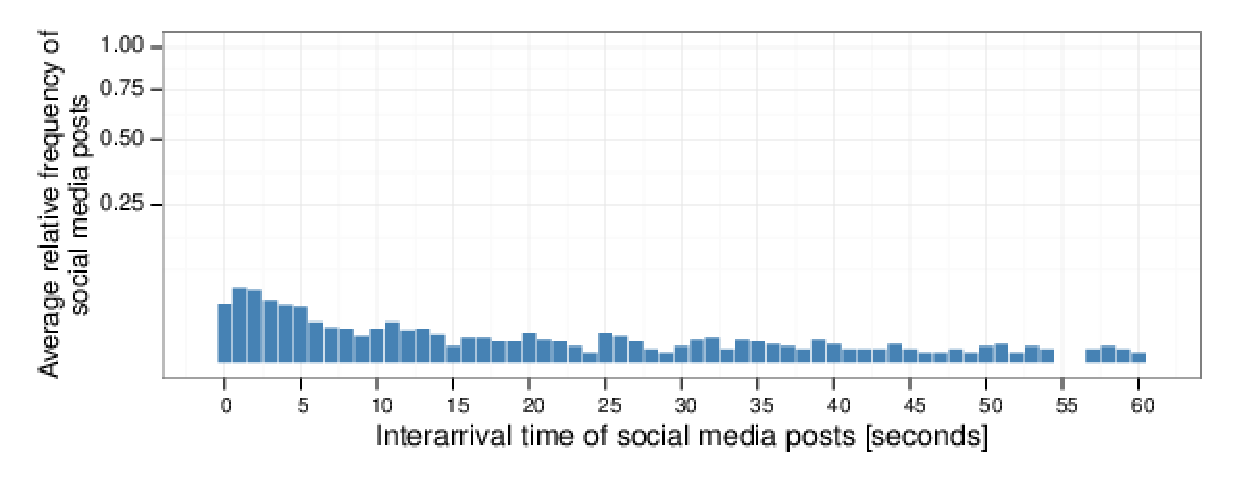
\includegraphics[width=\textwidth]{figures/plots_revision/fig1b}
%    \caption{User posts about The Oscars arriving several weeks before
%      the event.}
%    \label{fig:fig1b}
%  \end{subfigure}%
%  ~ %add desired spacing between images, e. g. ~, \quad, \qquad, \hfill etc.
%  % (or a blank line to force the subfigure onto a new line)
%
%  \caption{\textbf{Examples of interarrival time histograms of two real-world news
%events discussed on Twitter. The event [nelson, mandela] (Fig~\ref{fig:fig1a}) was
%      collected on 12/05/2013. Since there is a high
%      concentration in the first histogram bin, we conclude that most of the social media posts
%      for this event occur in one or more successions of high-activity
%      bursts (therefore, considered a high-activity event).
%      The second event, [may, oscar] (Fig~\ref{fig:fig1b}) was collected
%      on 03/23/2014 about The Oscars event that was held a few
%      weeks before. The arrival times of these posts are much more spread
%      out, displaying much less concentration of bursty activity.} 
%  }
%  \label{fig:fig1}
%\end{figure}
%
\begin{figure}[!htb]
  \centering
%    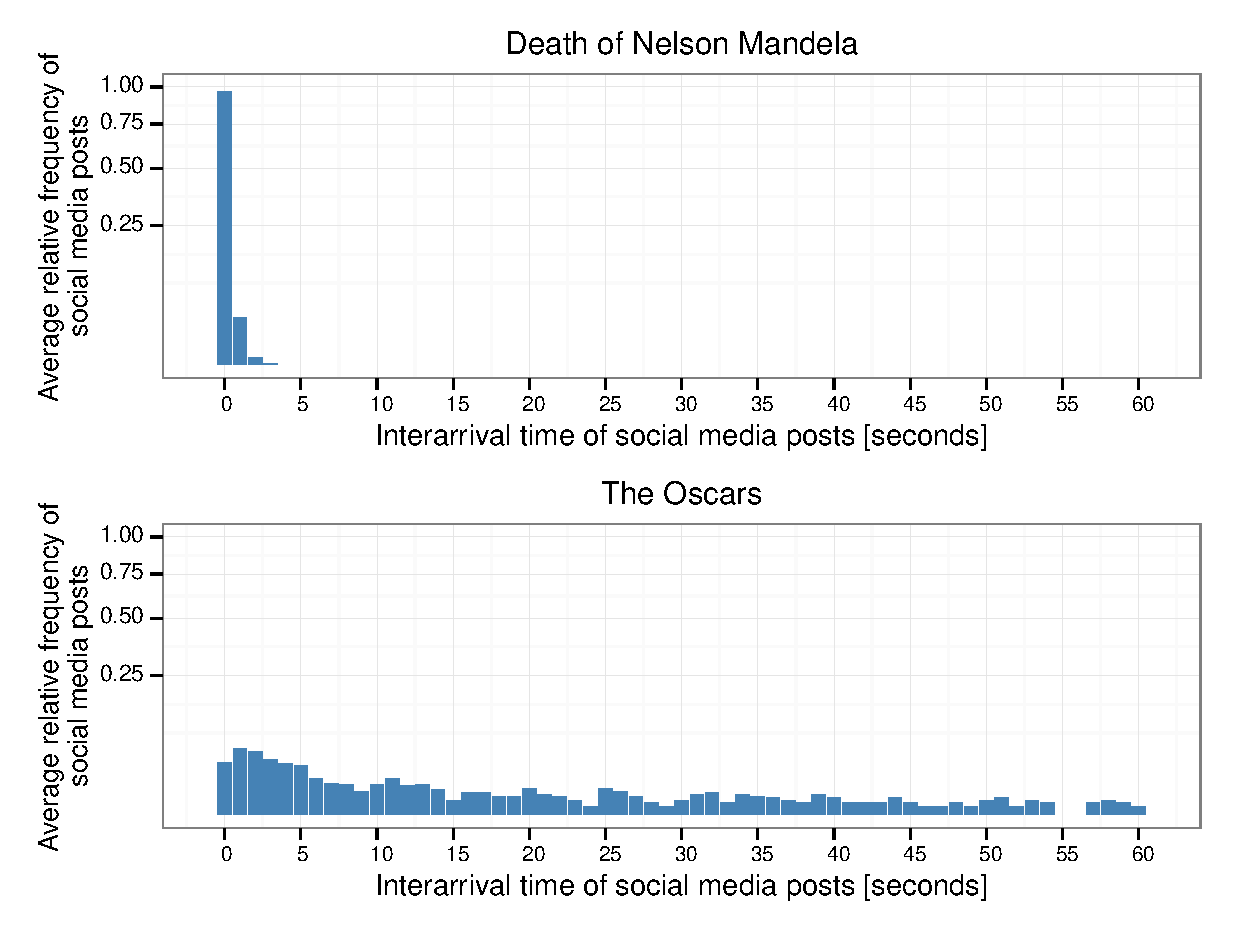
\includegraphics[width=\textwidth]{figures/plots_revision/fig1}
  \caption{\textbf{Examples of interarrival time histograms of two real-world news
events discussed on Twitter. The event [nelson, mandela] (top) was
      collected on 12/05/2013. Since there is a high
      concentration in the first histogram bin, we conclude that most of the social media posts
      for this event occur in one or more successions of high-activity
      bursts (therefore, considered a high-activity event).
      The second event, [may, oscar] (bottom) was collected
      on 03/23/2014 about The Oscars event that was held a few
      weeks before. The arrival times of these posts are much more spread
      out, displaying much less concentration of bursty activity.} 
  }
  \label{fig:fig1}
\end{figure}


We note that, by using interarrival times to describe the intensity of the
activity of an event, we make our analysis independent of the particular
evolution of each event. By doing this, we put no restrictions on how
high-activity events unfold in time, for example, they could be: (a) events
that start out slowly and
suddenly gain momentum, (b) events that go viral soon after they appear on
social media and then decay in intensity over a long (or short) period of
time, (c) events that from the beginning produce large amounts of interest and
sustain that interest throughout their long (or short) lifespan, or (d)
events that are a concatenation of any of the above, etc.

%\newtext{ 
% Experimental analysis

We study a dataset of news events gathered from news
headlines from a \emph{manually curated} list of well-known news media
accounts (e.g., @CNN, @BreakingNews, @BBCNews, etc.) in the
microblogging platform Twitter \cite{Twitter_website}
%\footnote{\url{https://twitter.com}
%  (Accessed: August 25, 2015.)} 
(a full list of all the news media
accounts is provided in the supplementary material). Headlines were
collected periodically every hour, over the course of approximately
one year. In parallel, all the Twitter messages (called \emph{tweets})
were extracted for each news event using the public
API \cite{Twitter_API}.
%\footnote{\url{https://dev.twitter.com/} (Accessed: August 25,
%  2015.)},
% In this research, since we focus on the microblogging platform
% Twitter, we collected all the Twitter messages (called
% \emph{tweets}) produced about each news event using the publicly
% available Twitter Search API
This process was performed by automatically extracting descriptive
sets of keywords for each event using a variation of frequent itemset
extraction \cite{Tan_Steinbach_Kumar} over the event's headlines.
These sets of keywords were then used to retrieve corresponding user
tweets for each event. We validate the events gathered in our
data collection process to ensure that each group of social media
posts corresponds to a meaningful and cohesive news event. We provide a detailed
description of the collection methodology and of the validation of event
cohesiveness in the supplementary material. Overall, the resulting dataset contains
$43,256,261$ tweets that account for $5,234$ events (Table~\ref{table:dataset-stats}).

In Fig~\ref{fig:fig2} we characterize an example event from our
dataset, by showing the set of keywords and a sample of tweets
associated to the event. These keywords form a semantically meaningful
event; they refer to the incident where soccer player Luis Suarez was
charged for biting another player during the FIFA World Cup in
2014. This general collection process results in a set of social media
posts associated to an event which can encompass several memes, viral
tweets and pieces of information. Therefore, an event is composed of
diverse information, addressing more heterogeneous content than prior
work
% \cite{Castillo:2014},\cite{Szabo:2010},\cite{Lerman:2010},\cite{Tatar:2011},\cite{Pinto:2013},\cite{Ahmed:2013,
% Zaman_information_spreading},\cite{suh2010want}
\cite{Castillo:2014,Szabo:2010,Lerman:2010,Tatar:2011,Pinto:2013,Ahmed:2013,suh2010want}
which focus on single pieces of information (e.g., a
particular meme, a viral tweet etc.).
\begin{table}[!htb]
  \centering
  \begin{tabularx}{\textwidth}{@{}p{6cm}llll@{}}
    \toprule
    \textbf{Event Collection Statistics} & \textbf{Minimum} & \textbf{Mean} & \textbf{Median} & \textbf{Maximum} \\ \midrule
    \# of posts (per event) & 1,000 & 8,254 & 2,474 & 510,920 \\
    \# of keywords (per tweet) & 2 & 3.77 & 3 & 39 \\
    Event duration (hours) & 0.12 & 20.93 & 7.46 & 190.43 \\ \bottomrule
  \end{tabularx}
  \caption{\bf High-level description of the dataset of news events.} \label{table:dataset-stats}
\end{table}

\begin{figure}[!htb]
%    \includegraphics[width=\textwidth]{figures/plots_revision/fig2}
  \caption{\textbf{An example event, collected on 06/25/2014
      with keywords (left) and sample user posts (right) obtained
      from the Twitter Search API. The tweets in the event contain at
      least a pair of descriptive keywords and were retrieved close to the time
      of the event.}}
  \label{fig:fig2}
\end{figure}

The collection of events is converted into their VQ-event model
representation. Using this model, we can identify events that have
produced similar levels of activity in the social network. In other
words, events are considered to have similar activity if the
interarrival times between their social media posts are similarly
distributed, implying a very much alike collective reaction from users
to the events within a group. In order to identify groups of similar
events, we cluster the event models. We sort the resulting groups of
events from highest to lowest activity, according to the concentration
of social media posts in the bins that correspond to short
interarrival times. We consider the events that fall in the top
cluster to be high-activity events as most of their interarrival times
are concentrated in the smallest interval of the VQ-event model.  In
our dataset, these correspond to roughly 8\% of the events.  We
consider the next clusters in the sorted ranking to form medium-high
activity events, and so on.  Thus we end with four groups of events:
high, medium-high, medium-low and low. Fig~\ref{fig:fig3} shows a
heatmap of the interarrival relative frequency for each cluster. This
classification of events based on activity intensity is independent of
event size. More details of this methodology are provided in S1 Appendix.

\begin{figure}[!htb]
%    \includegraphics[width=\textwidth]{figures/plots_revision/fig3}
  \caption{\textbf{Each row is the average representation of all the
      events in a cluster.  A darker cell represents a higher
      relative frequency value.  The y-axis specifies the number of events in
      each
      cluster.  Clusters are (top to bottom): high-activity, medium-high
      medium-low and low.}
    % \inote{Mauricio: change labels of x and y-axis (to: Event type
    % (total number of events))}
  }
  \label{fig:fig3}
\end{figure}

% Results and Discussion can be combined.
\section*{Results and Discussion}
%\newtext{ 
Our main objective in this work is to analyze the
  characteristics of high-activity events which differentiate them from
  other types of events. In particular, we identify how early on in an
  event's lifecycle can we determine if an event is going
  produce high activity in the on-line social network.

Tables~\ref{table:high-impact-sample}
and~\ref{table:low-impact-sample} show examples of events from the
high-activity category and low-activity category. We recall that the
high-activity events are those which were in the top 8\% of the
ranking obtained by sorting the event clusters according to
concentration of interarrival times of social media posts in the
shortest interarrival time of the VQ-event model.  Table
\ref{table:high-impact-sample} shows two events of different sizes
(large and small) and different scopes (one global and the other of
more local scope) categorized as high activity in our dataset. The
first event, the death of Nelson Mandela, is one of the largest events
in the dataset, with $\approx 134,000$ tweets. The histogram
representation of this event, shown in Fig~\ref{fig:fig1}, suggests
that more than $80\%$ of the activity of the event was produced in
high-activity periods.  This is an event of international, political,
and social importance, that produced an overwhelming flood of messages
on social media. %% add detail about reach and scope 
Hence, it makes
sense for such an example to be a high-activity event.  The second
event, on the other hand, about the 2013 Mumbai Gang Rape is of much
smaller scale, with a total of $\approx 1,700$ tweets.  However, this
event caused considerable amount of immediate reaction on social
media, with close to $50\%$ of its activity concentrated within
high-activity periods. Despite its smaller size, in comparison to the
previous event, this event displays a similar reaction to that of
other high-activity events, but at a smaller scale. 
%More detailed
%inspection of the event shows that geolocated users which discussed
%this event were mostly from India and the U.K. In addition, we find
%that in the following days other events that are repercussions of this
%event gather a great deal of attention (with $\approx 12,700$
%tweets). % is it good to include this fact??

Table \ref{table:low-impact-sample} shows events that have been
classified by our methodology in the category of low activity.  The
first event, about a teen surviving after hiding in the wheel of a
airplane, had only a little more than $25\%$ of its messages arriving
with high-activity bursts although it had over $18,000$ messages.  The
second event, about the damages caused by a tornado in Canada, did not
garner much immediacy in attention of Twitter users, with only $7\%$
of its messages produced with short interarrival times. Most of the
messages of this event were well spaced out in time. Even though we
cannot say whether or not this event had significant implications in
the real-world, we can say that it did not have considerable impact on
the Twitter network. The lack of interest could be due to several
factors that are currently beyond the scope of this work, ranging from
the lack of Twitter users in the locality of the real-world event, to
it not being considered urgent by Twitter users. We intend to research
the relation between the real-world impact of an event and the network
reaction in future work.


%%%%%%%%% REWRITE ANALYSIS OF HISTOGRAM DISTRIBUTIONS %%%%%%%%%%%%

% Fig.~\ref{fig:highest}, Fig.~\ref{fig:low}, Fig.~\ref{fig:cdf-highest} and
% Fig.~\ref{fig:cdf-lowest} show the average histograms and the average
% cumulative distribution functions of the events corresponding to the
% high and low activity categories, respectively.  Visually, the average
% high-activity event vector representations starkly differ from that of
% a low-activity event in that the histogram in Fig.~\ref{fig:highest}
% seems to possess an exponential decay, while the histogram in
% Fig.~\ref{fig:low} does not.  To test this hypothesis, we fit
% exponential function of the form $f(x)=ae^{bx}$ to the event
% histograms. Table~\ref{tab:curve_fitting} summarizes the results from
% statistical significance tests performed on the parameters $a$ and
% $b$, and on the residual least squares error used for fitting the
% exponential curves.  The differences between these values is
% statistically significant ($p$-value $\leq2.2\times 10^{-16}$), thus demonstrating
% that high-activity events, on an average, fit the exponential decay
% curve much better than their low-activity counterparts.  In addition,
% Fig.~\ref{fig:param_est} shows two scatter plots with the resulting
% exponential parameters $a$ and $b$.  We observe that the majority
% ($97.4\%$) of high-activity events have an exponent $b \leq -50$,
% separating them unequivocally from other events.

%}


Fig~\ref{fig:fig4} shows the average histograms for events that
belong to the high activity, medium-high activity, medium-low activity
and low-activity clusters (displayed from left to right and top to
bottom). All histograms show a quick decay in average relative
frequency (resembling a distribution from the exponential family). In
particular, the high-activity group concentrates most of its activity
in the shortest interarrival rate, with lower activity groups mostly
concentrating their activity in the second bin with slower
decay. Fig~\ref{fig:fig5} further characterizes the differences in
behavior of the high and low-activity groups, showing that
high-activity events concentrate on average $70\%$ fo their activity
in the smallest bin ($0$ sec.), against $8\%$ for low-activity
events. In addition, Fig~\ref{fig:fig6} (left) shows the cumulative
distribution function (CDF) for each group of events, and
Fig~\ref{fig:fig6} (right) shows $\log{(1 - \mathrm{CDF})}$. Visual
inspection shows a clear difference in how interarrival rates are
distributed within each group, however, these figures do not indicate a
power-law distribution nor exponential distribution.%%

%%% Table with example tweets for events
\begin{table}[!htb]
  \centering
  {\scriptsize
    \begin{tabular*}{1\linewidth}{p{5cm}p{5cm}}
      \toprule
      \textbf{Event} & \textbf{Sample Tweets} \\
      \midrule
      \pbox{20cm}{\textbf{Description:}\\ Death of South African\\ politician Nelson Mandela. \vspace{.1cm}\\
        \textbf{Keywords:}\\ {[}nelson, mandela{]}\vspace{.1cm}\\
        \textbf{Date:}\\ 2013-12-05 \vspace{.1cm}\\
        \textbf{Size:} \\ 134,637 tweets}
      & \pbox{20cm}{
        @DaniellePeazer: RIP Nelson Mandela..... what a truly phenomenal and\\ inspirational man xx\vspace{.1cm}\\
        @iansomerhalder: Im in tears.The world has lost one of its greatest shepherds \\of peace. Thank you Mr.Mandela for the love you radiated. http://t.co/u39MVVEKe8\vspace{.1cm}\\
        @FootballFunnys: This is so true. RIP Nelson Mandela. http://t.co/vF9xri8LdP\vspace{.1cm}\\
        @David\_Cameron: I've spoken to the Speaker and there will be statements \\and tributes to Nelson Mandela in the House on Monday.} \\
      \midrule
      \pbox{20cm}{\textbf{Description:}\\ 2013 Mumbai Gang Rape \vspace{.1cm}\\
        \textbf{Keywords:}\\ {[}rape, mumbai{]}\vspace{.1cm}\\
        \textbf{Date:}\\ 2013-08-24 \vspace{.1cm}\\
        \textbf{Size:} \\1,705 tweets}
      & \pbox{20cm}{
      % select user.screen_name, text from tweet join user on tweet.user_id_id = user.user_id where event_id_id = 272;
      @TheNewsRoundup: Mumbai gang-rape: Second accused confesses to crime: \\Mumbai Police - Daily News Analysis http://t.co/KnabwhqH66\vspace{.1cm}\\
      @vijayarumugam: An interesting take on the Mumbai rape: http://t.co/ylBmW4l8sA\vspace{.1cm}\\
      @LondonStephanie: Two arrested over gang rape of Mumbai photojournalist \\that sparked renewed protests in India http://t.co/McYfLNDvaE\vspace{.1cm}\\
      @GanapathyI: Most brutal rapist of Delhi gang-rape was 17. Most brutal rapist\\ of Mumbai gang-rape is 18. Worst Young generation I have seen in my life.}\\
%        @M\_arioBalotelli: CLEAR ANGLE of the Suarez bite!!  https://t.co/bI08YsZWSE\vspace{.1cm}\\
%        @fifamedia: Disciplinary proceedings opened against Uruguay's Luis Suarez\\ http://t.co/w6mRNuSGZt\vspace{.1cm}\\
%        @DeadlineDayLive: Luis Suarez will sign a 5-year contract at Barcelona and he'll wear \\the no. 9 shirt. (Source: http://t.co/6uRIUwjsGN) http://t.co/FxyOf9ERVr\vspace{.1cm}\\
%        @GeniusFootball: BREAKING: FIFA have caught Suarez leaving the stadium?\\ http://t.co/vsQQCVV1GQ} \\
      \bottomrule
    \end{tabular*}
  }
  \caption{\textbf{
        Examples of high-activity news events. The events
      shown were taken from the ``high'' category according to
Fig.~\ref{fig:fig4}.
        }}
  \label{table:high-impact-sample}
\end{table}

\begin{table}[!htb]
  \centering
  {\scriptsize
    \begin{tabular*}{1\linewidth}{p{5cm}p{5cm}}
      \toprule
      \textbf{Event} & \textbf{Sample Tweets} \\
      \midrule
      \pbox{20cm}{\textbf{Description:}\\Teen survives hiding \\in a plane wheel.\vspace{.1cm}\\
        \textbf{Keywords:}\\ {[}teen, survives, old, \\well, skydivers, plane, wheel, flight{]}\vspace{.1cm}\\
        \textbf{Date:}\\ 2014-04-21 \vspace{.1cm}\\
        \textbf{Size:}\\ 18,519}
      & \pbox{20cm}{
        %select user.screen_name, text from tweet join user on tweet.user_id_id = user.user_id where event_id_id in (22310,22274,22240);
        @ToniWoemmel: 16-year-old somehow survives flight from California to\\ Hawaii stowed away in planes wheel well: http://t.co/IGiJa60SiK\vspace{.1cm}\\
        @iOver\_think: 38,000 feet at -80F: Teen stowaway survives five-hour\\ California-to-Hawaii flight in wheel well http://t.co/ejXQH9VZyT\vspace{.1cm}\\
        @TruEntModels: GOD IS GOOD...runaway TEEN hid in plane's wheel for\\ 5 HOUR flight during FREEZING temps and survived http://t.co/6g6Cqhs9Ib\vspace{.1cm}\\
        @DvdVill: A 16-year-old kid, who was mad at his parents, hid inside a jet\\ wheel and survived flight to Hawaii. http://t.co/c82GbjrfUH\\
        %@guardiannews: Angela Merkel denied access to her NSA file http://t.co/FLQc0zSjYJ\vspace{.1cm}\\
        %@mog7546: \#GERMANY's \#Merkel says \#OBAMA's \#US assurances on \#NSA spying\\ "INSUFFICIENT" - Reuters India http://t.co/D2L52CP9YZ\vspace{.1cm}\\
        %@GermanyForum: Merkel denied access to own NSA file http://t.co/e6vKCOkbXA\vspace{.1cm}\\
        %@kgosztola: US ignores request from German Chancellor Angela \\Merkel to look at NSA file:\\ http://t.co/HFTMMZBu5W
      }
      \\
            \midrule
      \pbox{20cm}{\textbf{Description:}\\Surveying the damages of \\ recent tornado in Canada. \vspace{.1cm}\\
        \textbf{Keywords:}\\ {[}canada, tornado{]}\vspace{.1cm}\\
        \textbf{Date:}\\ 2014-06-21 \vspace{.1cm}\\
        \textbf{Size:}\\ 1,033}
      & \pbox{20cm}{
        @Kathleen\_Wynne: Visited \#Angus today to survey the damage. Thankfully no \\fatalities or major injuries from recent tornado. http://t.co/xRQyRWg5Vw\vspace{.1cm}\\
        @SunNewsNetwork: PHOTOS \& VIDEO: Hundreds displaced after \\ tornado hits Ontario town, destroying homes http://t.co/L38rG6N1a6\vspace{.1cm}\\
        @CBCToronto: Kathleen Wynne is speaking at site of tornado damage in Angus, \\Ont. now. Watch live here: http://t.co/EDKNUiZo0X \#cbcto\vspace{.1cm}\\
        @InsuranceBureau: @CTVBarrieNews: Insurance Bureau of Canada is setting up \\a mobile unit in \#Angus today to help residents affected by \#Tornado}
      \\
      \bottomrule
    \end{tabular*}
  }
  \caption{\textbf{
                Examples of events with low activity. The events
      shown were taken from the ``low'' category according to
Fig.~\ref{fig:fig4}}
          .}
  \label{table:low-impact-sample}
\end{table}

%\input{events_example_PLOS_revision}

\begin{figure}[!htb]
  \centering
%    \includegraphics[width=\textwidth]{figures/plots_revision/fig4}
  \caption{\textbf{Average histograms of the high activity,
      medium-high activity, medium-low activity and low activity
      clusters in our dataset (from left to right and top to
      bottom). All histograms include standard deviation bars and were
      cut-off at 60 second length for better visibility.
      % \inote{change labels of x and y axis}
    }}\label{fig:fig4}
\end{figure}

\begin{figure}[!htb]
  \centering
%    \includegraphics[width=\textwidth]{figures/plots_revision/fig5}
  \caption{\textbf{Scatter plots of the average relative frequencies of interarrival times
for the high-activity and low-activity clusters of events (i.e., scatter
plots of the histograms in Fig~\ref{fig:fig4} in log-log scale). $y$-axis
represents the average relative frequency of social media messages and
$x$-axis the interarrival time.
    }}\label{fig:fig5}
\end{figure}

\begin{figure}[!htb]
  \centering
% \includegraphics[width=\textwidth]{figures/plots_revision/fig6_log}
  \caption{\textbf{(Left) Average cumulative distribution function (CDF) for
the high activity, medium-high activity, medium-low activity and low activity clusters in our dataset.
(Right) $\log{(1 - \mathrm{CDF})}$ for the same clusters. 
      % \inote{change labels of x and y axis}
    }}\label{fig:fig6} %% fig6_long_inf_omitted.pdf
\end{figure}

Further analysis of the high-activity events shows significant
differences to other events, in the following aspects: (i) how the
information about these events is propagated, (ii) the characteristics
of the conversations that they generate, and (iii) how focused users
are on the news topic. In detail, high-activity events have a higher
fraction of {\em retweets} (or shares) relative to their overall
message volume. On average, a tweet from a high-activity event is
retweeted 2.36 times more than a tweet from a low activity event. The
most retweeted message in high-activity events is retweeted 7 times more
than the most retweeted message in a medium or low activity event. We
find that a small set of initial social media posts are propagated
quickly and extensively through the network without any rephrasing by
the user (just plain forwarding). Intuitively, this seems justified given
general topic urgency of high-activity events. Events that are not
high-activity did not exhibit these characteristics.

Our research also revealed that high-activity events tend to spark more conversation
between users, 33.4\% more than other events. This is reflected in the
number of {\em replies} to social media posts. The number of different
users that engage with high-activity events is 32.7\% higher than in
events that are not high-activity. Posts about high-activity events are
much more topic focused than in other events. The vocabulary of unique
words as well as {\em hashtags} used in high-activity events is much
more narrow than for other events. Medium and low activity events have
over 7 times more unique hashtags than high-activity events. This is
intuitive, given that if a news item is sensational, people will
seldom deviate from the main conversation topic.

% We have presented an analysis of high-impact news events based on
% the data of their entire life-cycle in the social network. We used
% the arrival time intervals to create a model that allows us to
% classify the event according to its impact. Nevertheless,

In a real-world scenario, in order to predict if an early breaking
news story will have a considerable impact in the social network, we
will not have enough data to create its activity-based model, i.e., we
will not yet know the distribution of the speed at which the social
media posts will arrive for the event. For instance, an event can
start slowly and later produce an explosive reaction, or start
explosively and decay quickly to an overall slower message arrival
rate. Still, reliable early prediction of very high-activity news is
important in many aspects, from decisions of mass media information
coverage, to natural disaster management, brand and political image
monitoring, and so on.

For the task of early prediction of high-activity events we use features 
that are independent of our activity-based model such as
the retweets, the sentiment of the posts about the event, etc. 
These features are computed on the early 5\% of messages about the event.
% More details are provided in the supplementary material.
The results are an average from a 5-fold cross validation with
randomly selected 60\% training, 20\% validation and 20\% test splits.
The high-activity events are identified with a precision of 82\% using
only the earliest 5\% of the data of each event
(Table~\ref{tab:classification_results}).  Additionally, we were able to
identify with high accuracy a considerable percentage of all
high-activity events ($\approx 46\%$) at an early stage, with very few
false positives (Table~\ref{tab:classification_results} and~\ref{tab:confusion_matrix}).

\begin{table}[!htb]
  %\begin{adjustwidth}{-10mm}{-10mm}
  \centering
  {\small
    \begin{tabularx}{\textwidth}{lcccc|cccc}
      \toprule
      & \multicolumn{4}{c}{\textbf{Early 5\% Tweets}} & \multicolumn{4}{c}{\textbf{All Tweets}} \\
      \midrule
      & FP-Rate & Precision & Recall & ROC-area & FP-Rate & Precision & Recall & ROC-area \\
      % \midrule
      high-activity & 0.009 & 0.819 & 0.455 & 0.900 & 0.01 & 0.830 & 0.540 & 0.945 \\
      non-high-activity & 0.545 & 0.954 & 0.991 & 0.900 &  0.460 & 0.960 & 0.990 & 0.945 \\
      \bottomrule
    \end{tabularx}
  }
  \caption{\textbf{Classification of high-activity events.}}
  \label{tab:classification_results}
  %\end{adjustwidth}
%                                                                                                                                448,1         93%
\end{table}

\begin{table}[!htb]
  \centering
  % {\scriptsize
  \begin{tabularx}{\textwidth}{lcc|cc}
    \toprule
    \multirow{2}{*}{ }& \multicolumn{2}{c}{\textbf{Early 5\% Tweets}} & \multicolumn{2}{c}{\textbf{All Tweets}} \\
    \midrule
    % \cmidrule{2-5} \cline{2-5}
    & high-activity & non-high-activity & high-activity & non-high-activity \\
    % \midrule
    high-activity & $194$ & $232$ & $230$ & $196$\\
    non-high-activity & $43$ & 4,765 & 47 & 4,761 \\
    \bottomrule
  \end{tabularx}
  % }
  \caption{\textbf{Confusion matrix for high-activity events prediction.}}
  \label{tab:confusion_matrix}
\end{table}



The precision using only the early tweets is almost as good as using
all tweets in the event (0.819 to 0.830). This suggests that the
social network somehow acts as a natural filter in separating out the
high-activity events fairly early on.  The recall goes from 0.455 to
0.540. This indicates that there are some high-activity events which
require more data in order to determine what kind of activity they will
produce, or events for which activity occurs due to random conditions. A
detailed description of the features and different classification
settings are provided in the supplementary material.%\supplementary.




\section*{Conclusion}

We study the characteristics of the activity that real-world news produces
in the Twitter social network. In particular, we propose to measure the impact of the
real-world news event on the on-line social network by modeling the user
activity related to the event using the distribution of their
interarrival times between consecutive messages. In our research we observe
that the activity triggered by real-world news events follows a similar
pattern to that observed in other types of collective reactions to events.
This is, by displaying periods of intense activity as well as long periods of
inactivity. We further extend this analysis by identifying groups of events
that produce much more concentration of high-activity than other events. 
We show that there are several specific properties that distinguish how
high-activity events evolve in Twitter, when comparing them to other
events. We design a model for events, based on the codebook approach, that allows us to do
unambiguous classification of high-activity events based on the impact
displayed by social network. % This definition does not have some of the
%problems that current notions of virality and popularity have. 
Some notable
characteristics of high-activity events are that they are forwarded more
often by users, and generate a greater amount of conversation than
other events.  Social media posts from high-activity news events are
much more focused on the news topic. Our experiments show that there
are several properties that can suggest early on if an event will have
high-activity on the on-line community.  We can predict a high number of
high-activity events {\em before} the network has shown any type of
explosive reaction to them. % Using simple off-the-shelf feature based
%classifiers, we can
% predict many high-impact events with high precision.
This suggests that users are collectively quick at deciding whether an
event should receive priority or not.  However, there does exist a fraction of
events which will create high activity, despite not presenting
patterns of other high activity events during their early stages.  These
events are likely to be affected by other factors, such as random
conditions found in the social network at the moment and require
further investigation.

\section*{Supporting Information}
\subsection*{S1 Appendix}

\section*{Acknowledgements}
We thank Gonzalo Navarro (U Chile), 
Jeanna Matthews (Clarkson Univ.) and Vanessa Murdock (Microsoft) 
and the reviewers for their valuable feedback and comments.


\nolinenumbers

%\section*{References}
\bibliographystyle{plain}

\begin{thebibliography}{10}

\bibitem{Kwak:2010}
Kwak H, Lee C, Park H, Moon S.
\newblock What is Twitter, a Social Network or a News Media?
\newblock In: Proceedings of the 19th International Conference on World Wide
  Web. WWW '10. New York, NY, USA: ACM; 2010. p. 591--600.
\newblock Available from: \url{http://doi.acm.org/10.1145/1772690.1772751}.

\bibitem{Castillo:2014}
Castillo C, El-Haddad M, Pfeffer J, Stempeck M.
\newblock Characterizing the Life Cycle of Online News Stories Using Social
  Media Reactions.
\newblock In: Proceedings of the 17th ACM Conference on Computer Supported
  Cooperative Work and Social Computing. CSCW '14. New York, NY, USA: ACM;
  2014. p. 211--223.
\newblock Available from: \url{http://doi.acm.org/10.1145/2531602.2531623}.

\bibitem{Szabo:2010}
Szabo G, Huberman BA.
\newblock Predicting the Popularity of Online Content.
\newblock Commun ACM. 2010 Aug;53(8):80--88.
\newblock Available from: \url{http://doi.acm.org/10.1145/1787234.1787254}.

\bibitem{Lerman:2010}
Lerman K, Hogg T.
\newblock Using a Model of Social Dynamics to Predict Popularity of News.
\newblock In: Proceedings of the 19th International Conference on World Wide
  Web. WWW '10. New York, NY, USA: ACM; 2010. p. 621--630.
\newblock Available from: \url{http://doi.acm.org/10.1145/1772690.1772754}.

\bibitem{Tatar2014}
Tatar A, de~Amorim MD, Fdida S, Antoniadis P.
\newblock A survey on predicting the popularity of web content.
\newblock Journal of Internet Services and Applications. 2014;5(1):1--20.
\newblock Available from: \url{http://dx.doi.org/10.1186/s13174-014-0008-y}.

\bibitem{Pinto:2013}
Pinto H, Almeida JM, Gon\c{c}alves MA.
\newblock Using Early View Patterns to Predict the Popularity of Youtube
  Videos.
\newblock In: Proceedings of the Sixth ACM International Conference on Web
  Search and Data Mining. WSDM '13. New York, NY, USA: ACM; 2013. p. 365--374.
\newblock Available from: \url{http://doi.acm.org/10.1145/2433396.2433443}.

\bibitem{Ahmed:2013}
Ahmed M, Spagna S, Huici F, Niccolini S.
\newblock A Peek into the Future: Predicting the Evolution of Popularity in
  User Generated Content.
\newblock In: Proceedings of the Sixth ACM International Conference on Web
  Search and Data Mining. WSDM '13. New York, NY, USA: ACM; 2013. p. 607--616.
\newblock Available from: \url{http://doi.acm.org/10.1145/2433396.2433473}.

\bibitem{Li:2016:concept:drift}
Li CT, Shan MK, Jheng SH, Chou KC.
\newblock Exploiting Concept Drift to Predict Popularity of Social Multimedia
  in Microblogs.
\newblock Inf Sci. 2016 Apr;339(C):310--331.
\newblock Available from: \url{http://dx.doi.org/10.1016/j.ins.2016.01.009}.

\bibitem{Liu:2015:UN}
Liu Q, Zhou M, Zhao X.
\newblock Understanding News 2.0.
\newblock Inf Manage. 2015 Nov;52(7):764--776.
\newblock Available from: \url{http://dx.doi.org/10.1016/j.im.2015.01.002}.

\bibitem{berger2012makes}
Berger J, Milkman KL.
\newblock What makes online content viral?
\newblock Journal of Marketing Research. 2012;49(2):192--205.

\bibitem{iribarren2011branching}
Iribarren JL, Moro E.
\newblock Branching dynamics of viral information spreading.
\newblock Physical Review E. 2011;84(4):046116.

\bibitem{guerini2011exploring}
Guerini M, Strapparava C, {\"O}zbal G.
\newblock Exploring Text Virality in Social Networks.
\newblock In: ICWSM; 2011. .

\bibitem{mills2012virality}
Mills AJ.
\newblock Virality in social media: the SPIN framework.
\newblock Journal of public affairs. 2012;12(2):162--169.

\bibitem{gaugaz2012predicting}
Gaugaz J, Siehndel P, Demartini G, Iofciu T, Georgescu M, Henze N.
\newblock Predicting the future impact of news events.
\newblock In: Advances in Information Retrieval. Springer; 2012. p. 50--62.

\bibitem{chile_elections}
{Telegraph}. Chile News;.
\newblock \url{http://www.telegraph.co.uk/news/worldnews/southamerica/chile/}.

\bibitem{ReisBOPKA15}
dos Reis JC, Benevenuto F, de~Melo POSV, Prates RO, Kwak H, An J.
\newblock Breaking the News: First Impressions Matter on Online News.
\newblock CoRR. 2015;abs/1503.07921.
\newblock Available from: \url{http://arxiv.org/abs/1503.07921}.

\bibitem{barabasi2005origin}
Barabasi AL.
\newblock The origin of bursts and heavy tails in human dynamics.
\newblock Nature. 2005;435(7039):207--211.

\bibitem{karsai2012universal}
Karsai M, Kaski K, Barab{\'a}si AL, Kert{\'e}sz J.
\newblock Universal features of correlated bursty behaviour.
\newblock Scientific reports. 2012;2.

\bibitem{gao2014quantifying}
Gao L, Song C, Gao Z, Barab{\'a}si AL, Bagrow JP, Wang D.
\newblock Quantifying information flow during emergencies.
\newblock arXiv preprint arXiv:14011274. 2014;.

\bibitem{yan2013information}
Yan Q, Wu L, Liu C, Li X.
\newblock Information propagation in online social network based on human
  dynamics.
\newblock In: Abstract and Applied Analysis. vol. 2013. Hindawi Publishing
  Corporation; 2013. .

\bibitem{ff}
Fei-Fei L, Perona P.
\newblock A Bayesian hierarchical model for learning natural scene categories.
\newblock In: Computer Vision and Pattern Recognition, 2005. CVPR 2005. IEEE
  Computer Society Conference on. vol.~2; 2005. p. 524--531 vol. 2.

\bibitem{Vaizman}
Vaizman Y, McFee B, Lanckriet G.
\newblock Codebook-based Audio Feature Representation for Music Information
  Retrieval.
\newblock IEEE/ACM Trans Audio, Speech and Lang Proc. 2014
  Oct;22(10):1483--1493.
\newblock Available from: \url{http://dx.doi.org/10.1109/TASLP.2014.2337842}.

\bibitem{Twitter_website}
{Twitter Inc };.
\newblock \url{https://www.twitter.com}.

\bibitem{Twitter_API}
{Twitter API};.
\newblock \url{https://dev.twitter.com}.

\bibitem{Tan_Steinbach_Kumar}
Tan PN, Steinbach M, Kumar V.
\newblock Introduction to Data Mining, (First Edition).
\newblock Boston, MA, USA: Addison-Wesley Longman Publishing Co., Inc.; 2005.

\bibitem{Tatar:2011}
Tatar A, Leguay J, Antoniadis P, Limbourg A, de~Amorim MD, Fdida S.
\newblock Predicting the Popularity of Online Articles Based on User Comments.
\newblock In: Proceedings of the International Conference on Web Intelligence,
  Mining and Semantics. WIMS '11. New York, NY, USA: ACM; 2011. p. 67:1--67:8.
\newblock Available from: \url{http://doi.acm.org/10.1145/1988688.1988766}.

\bibitem{suh2010want}
Suh B, Hong L, Pirolli P, Chi EH.
\newblock Want to be retweeted? large scale analytics on factors impacting
  retweet in twitter network.
\newblock In: Social computing (socialcom), 2010 ieee second international
  conference on. IEEE; 2010. p. 177--184.

\end{thebibliography}

\end{document}

